\documentclass[hyperref={pdfpagelabels=false},table,9pt,compress]{beamer}
% File Name: SetUp.tex
% Function: Make main settings of the document.


%%%%%%%%%%%%%%%%%%%%%%%%%%% BEGIN-Theme-settings %%%%%%%%%%%%%%%%%%%%%%%%%%
%%%%% http://www.hartwork.org/beamer-theme-matrix/
\usetheme{default} % Set the theme of the beamer.
%\usetheme{Frankfurt}                     %% Geovani style
%\setbeamercolor{alerted text}{fg=blue}   %% Geovani style
% W/o������:default, boxes, Bergen, Madrid, Pittsburgh, Rochester
% ���������:Antibes, JuanLesPins, Montpellier��
% ��Ŀ¼(TOC)�IJ�ߵ�����: Berkeley, PaloAlto, Goettingen, Marburg, Hannover��
% ��΢��frame������:Berlin, Ilmenau, Dresden, Darmstadt, Frankfurt, Singapore, Szeged��
% ����С�ڱ���: Copenhagen, Luebeck, Malmoe, Warsaw��
%\usecolortheme{default}  % Outer color themes. Alternatives: whale, seahorse, dolphin. default, beaver
\usecolortheme{orchid}  % Inner color themes. Alternatives: lily, orchid.
\useinnertheme[shadow]{rounded}
\usefonttheme{structurebold} % Font themes. Alternatives:  default, serif, structurebold, structureitalicserif, structuresmallcapsserif
\setbeamertemplate{frametitle}
{   \begin{center}
        \insertframetitle
    \end{center}
}
\setbeamertemplate{itemize items}[default] % Alternatives: default/triangle, circle, square, ball
\setbeamertemplate{enumerate items}[default] % Alternatives: default, circle, square, ball
\setbeamertemplate{navigation symbols}{}
\setbeamertemplate{footline}[frame number]
%\setbeamertemplate{footline}{%
%  \leavevmode%
%  \hbox{%
%    \begin{beamercolorbox}[wd=.333333\paperwidth,ht=2.25ex,dp=1ex,center]{author in head/foot}%
%      \usebeamerfont{author in head/foot}\insertshortauthor~(\insertshortinstitute)
%    \end{beamercolorbox}%
%    \begin{beamercolorbox}[wd=.333333\paperwidth,ht=2.25ex,dp=1ex,center]{title in head/foot}%
%      \usebeamerfont{title in head/foot}\insertshorttitle
%    \end{beamercolorbox}%
%    \begin{beamercolorbox}[wd=.333333\paperwidth,ht=2.25ex,dp=1ex,right]{date in head/foot}%
%      \usebeamerfont{date in head/foot}\insertshortdate{}\hspace*{2em}
%      \insertframenumber{} / \inserttotalframenumber \hspace*{2ex}
%    \end{beamercolorbox}
%    }%
%  \vskip0pt%
%}
%%%%%%%%%%%%%%%%%%%%%%%%%%%% END-Theme-settings %%%%%%%%%%%%%%%%%%%%%%%%%%%


%%%%%%%%%%%%%%%%%%%%%%%%%%%%%% BEGIN-Packages %%%%%%%%%%%%%%%%%%%%%%%%%%%%%
\usepackage{amsmath,amssymb,amsfonts}
\usepackage{mathrsfs}
\usepackage{color,xcolor}
\usepackage{graphicx,subfigure}
\usepackage{clock} % Use this package to insert a clock in the beamer.
\usepackage{textcomp}
\usepackage[T1]{fontenc}
\usepackage{verbatim}
\usepackage{moreverb}
\usepackage{multirow,multicol}
%\usepackage{url}
%\usepackage[colorlinks,linkcolor=blue,citecolor=blue,urlcolor=blue]{hyperref}%[colorlinks,linkcolor=blue,citecolor=blue,urlcolor=blue]
\usepackage{CJK}
%%%%%%%%%%%%%%%%%%%%%%%%%%%%%%%% END-Packages %%%%%%%%%%%%%%%%%%%%%%%%%%%%%


% \setbeamertemplate{navigation symbols}{} % Disable the buttons at the bottom.

\graphicspath{{Figures/}} % Set the directory where figures are saved.

%\AtBeginSection{
%  \begin{frame}{Outline}
%    \tableofcontents[currentsection,hideallsubsections]
%  \end{frame}
%}
%\AtBeginSubsection{
%  \begin{frame}{Outline}
%    \tableofcontents[currentsection,currentsubsection]
%  \end{frame}
%}
\AtBeginSection{
  \begin{frame}{Outline}
  \large{
  \tableofcontents[sections={\thesection}]  }
  \end{frame}
}

%%%%%%%%%%%%%%%%%%%% BEGIN-Theorem-like Environments %%%%%%%%%%%%%%%%%%%%%
\newtheorem{mybox}{}
\newtheorem{Con}{Conjecture}[section]
\newtheorem{Thm}{Theorem}[section]
\newtheorem{Prop}{Proposition}[Thm]
% show fig and table number
\setbeamertemplate{caption}[numbered]
% show theorems and example number
\setbeamertemplate{theorems}[numbered]
%%%%%%%%%%%%%%%%%%%%% END-Theorem-like Environments %%%%%%%%%%%%%%%%%%%%%%


%%%%%%%%%%%%%%%%%%%%%%%%%% BEGIN-New Commands %%%%%%%%%%%%%%%%%%%%%%%%%%%%
\newcommand{\email}[1]{Email: \href{mailto: #1}{\tt {\color{blue}#1}}}
\newcommand{\red}{\color{red}}
\newcommand{\blue}{\color{blue}}
\newcommand{\brown}{\color{brown}}
\newcommand{\orange}{\color{orange}}
\newcommand{\yellow}{\color{yellow}}
\newcommand{\Real}{\mathbb{R}}
\newcommand{\Tran}[1]{#1^\mathrm{T}}
\newcommand{\st}{\textnormal{s.t.}}
\newcommand{\dist}{\textnormal{dist}}
\newcommand{\bc}{\begin{center}}
\newcommand{\ec}{\end{center}}
\newcommand{\tbf}{\textbf}
\newcommand{\be}{\begin{equation}}
\newcommand{\ee}{\end{equation}}
\newcommand{\ba}{\begin{array}}
\newcommand{\ea}{\end{array}}
\newcommand{\btab}{\begin{table}\begin{tabular}}
\newcommand{\etab}{\end{tabular}\end{table}}
\newcommand{\nn}{\nonumber}
\newcommand{\xn}{x_1,x_2,\ldots,x_n}
\newcommand{\framee}[2]{\frame{\frametitle{#1} #2}}
\newcommand{\reff}[1]{(\ref{#1})} % ������
\newcommand{\inner}[2]{\left\langle#1,#2\right\rangle}

%\renewcommand{\baselinestretch}{1.3}
% Ĭ��������룬������ó����˶���
\renewcommand{\raggedright}{\leftskip=0pt \rightskip=0pt plus 0cm}
\raggedright
%\large
% define Roman numbers
\makeatletter
\newcommand{\rmnum}[1]{\romannumeral #1}
\newcommand{\Rmnum}[1]{\expandafter\@slowromancap\romannumeral #1@}
\makeatother
%%%%%%%%%%%%%%%%%%%%%%%%%%%% END-New Commands %%%%%%%%%%%%%%%%%%%%%%%%%%%%


\begin{document}
\begin{CJK*}{GBK}{kai}

\title[distance geometry]{\textsc{A New Error Function and Its Application in Distance Geometry Problem}}
\author[Zhenli SHENG]{Zhenli Sheng (ʢ����)\\email: {\blue szl@lsec.cc.ac.cn}}
% \institute{Institute of Computational Mathematics and Scientific/Engineering Computing}
\institute[ICMSEC, CAS]{Institute of Computational Mathematics and Scientific/Engineering Computing,\\Chinese Academy of Sciences}
\date[]{joint work with {\blue Prof. Ya-xiang Yuan} \\\textrm{} \\January 8, 2013\\ seminar talk}
\frame{
\titlepage
}

% File Name: ThankYou.tex
% Function: Insert an Outline page.


%\section*{\textsc{Outline}}
%\begin{frame}
%\frametitle{\textsc{Outline}}
%\end{frame}

\begin{frame}
\frametitle{\textsc{Outline}}
\tableofcontents%[pausesections]
\end{frame}


\transboxout

\section{Problem introduction}

\frame{
\frametitle{Distance Geometry Problem}
Find the coordinate vectors $x_{1},x_{2},\ldots,x_{n}$ that satisfy several given distances among them. Mathematically, this problem can be stated as following, \\

\newtheorem{myprob}{Distance Geometry Problem}
\begin{myprob}
\red{Find $x_{1},x_{2},\ldots,x_{n} \in \mathbb{R}^r$, such that
\begin{displaymath}
\|x_{i}-x_{j}\|=d_{ij},\quad (i,j) \in S.
\end{displaymath}
or
\begin{displaymath}
l_{ij}\leq \|x_{i}-x_{j}\|\leq u_{ij},\quad (i,j) \in S.
\end{displaymath}
}
\end{myprob}

\begin{itemize}
  \item The given data may have noise.
  \item This problem can be formulated as a global optimization problem.
  \item It has many applications.
\end{itemize}
}

\frame{
\frametitle{Global optimization: conventional error functions}
\begin{itemize}
  \item stress function
        \begin{equation*}
          Stress(x_{1},x_{2},\ldots,x_{n}) = \sum_{(i,j)\in S} (\|x_{i}-x_{j}\|-d_{i,j})^{2},
        \end{equation*}
  \item smoothed stress function
  \begin{equation*}
          SStress(x_{1},x_{2},\ldots,x_{n}) = \sum_{(i,j)\in S} (\|x_{i}-x_{j}\|^{{\red 2}}-d_{i,j}^{{\red 2}})^{2},
        \end{equation*}
  \item generalized stress function
        \footnotesize{
        \begin{equation*}
          GStress(x_{1},x_{2},\ldots,x_{n}) = \sum_{(i,j)\in S} \min\nolimits^{2} \{\frac{\|x_{i}-x_{j}\|^{2}-l_{i,j}^2}{l_{i,j}^{2}},0\} + \max\nolimits^{2} \{\frac{\|x_{i}-x_{j}\|^{2}-u_{i,j}^2}{u_{i,j}^{2}},0\}.
        \end{equation*} }
\end{itemize}
\vspace{4mm}
It has too many local minimizers, thus is very difficult to find the global solution.
}

\frame{
\frametitle{Application \Rmnum{1}: Graph Realization}
\begin{figure}
  \centering
  \subfigure{ 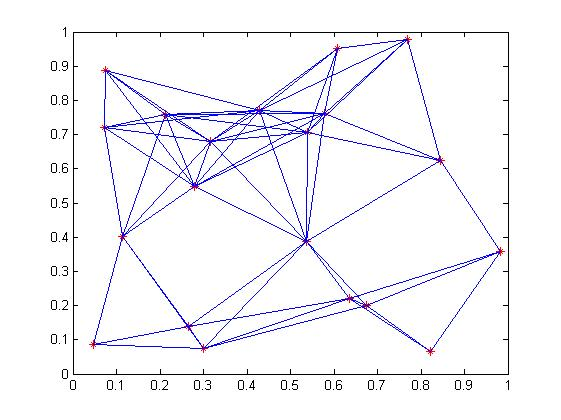
\includegraphics[width=5cm]{GraphRealization.jpg} }
  \subfigure{ 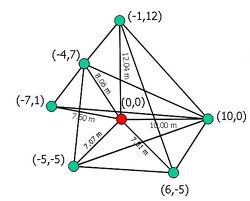
\includegraphics[width=5cm]{GraphRealization2.jpg} }
  \caption{ Graph Realization in 2D}
\end{figure}
\begin{center}
  Given a graph G=(V,E), each edge has a weight.
\end{center}
}

\frame{
\frametitle{{\red Application \Rmnum{2}: Protein Structure Determination}}
\begin{figure}[htp]
    \centering
    \subfigure{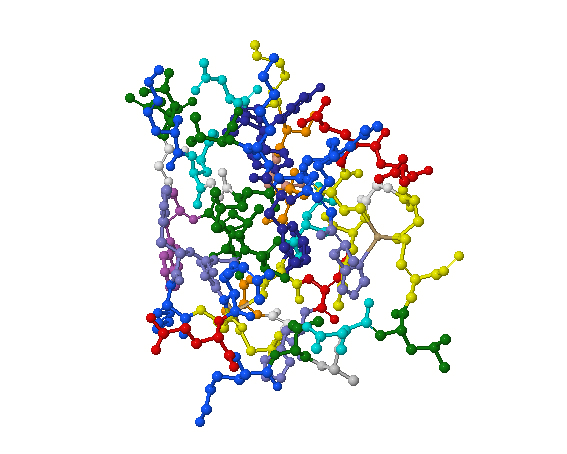
\includegraphics[width=5cm]{1PTQ2.jpg} }
    \subfigure{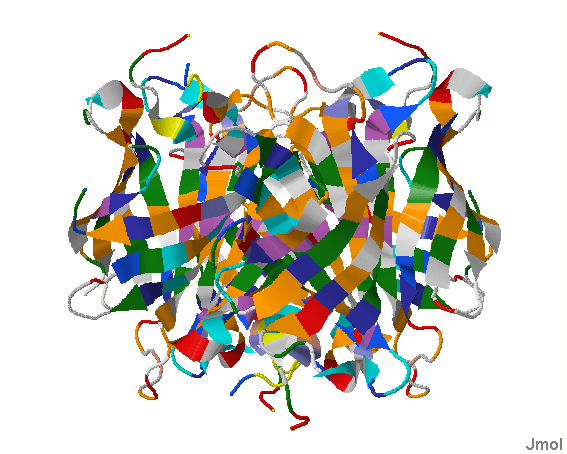
\includegraphics[width=5cm]{1HQQ2.jpg} }
    \caption{Two proteins: 1PTQ and 1HQQ, in different display ways}
\end{figure}
\begin{itemize}
\item 3D problem.
\item Measure distances by NMR or X ray crystallography.
\item Many properties of proteins rely on structure.
\end{itemize}
}

\frame{
\frametitle{Application \Rmnum{3}: Sensor Network Localization}
\begin{figure}[htp]
    \centering
    \subfigure{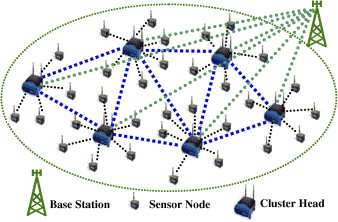
\includegraphics[width=4.5cm]{sensor2.jpg} }
    \subfigure{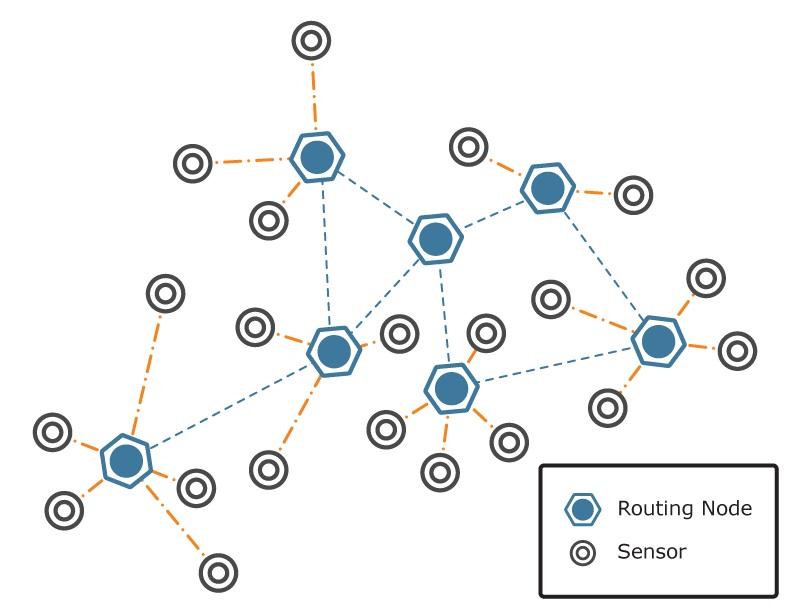
\includegraphics[width=4.5cm]{sensor1.jpg} }
    \caption{Illustration of wireless sensor networks: anchor and sensor}
\end{figure}
\begin{itemize}
  \item 2D problem.
  \item There are some anchors: locations are known.
\end{itemize}
}

\section{Related works review}
\subsection{Matrix decomposition method}
\frame{
\frametitle{Matrix Decomposition Method}
Matrix decomposition method {\blue [Blumenthal 1953, Torgerson 1958]} works for {\red Distance Geometry problem with full set of exact distances.} \\[3mm]
%\textrm{}\\
%\small{
Given a full set of distances, $d_{ij} = \| x_{i}-x_{j} \|, \quad i,j=1,2,\ldots,n.$
\begin{itemize}%[$\blacktriangleright$]
  \item Set $x_{n} = (0,0,0\Tran)$, thus $d_{in}=\|x_i\|$, we have
      \begin{eqnarray}
      % \nonumber to remove numbering (before each equation)
        \nonumber d_{ij}^{2} &=& \|x_{i}-x_{j}\|^{2} \\
        \nonumber             &=& \|x_{i}\|^{2}-2\Tran x_{i} x_{j}+\|x_{j}\|^{2} \\
                              &=& d_{in}^{2}-2\Tran x_{i} x_{j}+d_{jn}^{2}, \qquad  i,j=1,2,\ldots,n-1 \label{eq1}
      \end{eqnarray}
  \item Define $ X=(x_{1},x_{2},\ldots,x_{n}\Tran)$ and $D=\{(d_{in}^{2}-d_{ij}^{2}+d_{jn}^{2})/2: i,j=1,2,\ldots,n-1\}$,  (\ref{eq1}) $\Rightarrow {\red X\Tran X=D}$.
  \item Let $D=U\Sigma\Tran U$, $V=U(:,1:3)$ and $\Lambda=\Sigma(1:3,1:3)$. Then $X = V\Lambda^{1/2}$ is the best rank-3 approximation. [{\blue Eckart-Young 1936}]
\end{itemize}
}


\subsection{Buildup method}
\frame{
\frametitle{Buildup Method}
\begin{algorithm}[H]
\vspace{0.3cm}
Given: distance matrix D, i.e. $d_{ij}, (i,j)\in S$.
\begin{enumerate}[Step 1:]
  \item Find a clique of four points and determine their coordinates.
  \item Choose a point to be added, apply liner or nonlinear least square to locate the point.
  \item Repeat {\blue Step 2} until all points are determined or no more points can be determined.
\end{enumerate}
\caption{Buildup Method for Distance Geometry Problem with sparse data}
\end{algorithm}
\vspace{0.5cm}
$\spadesuit$ The algorithm bases on a simple observation: in $\mathbb{R}^3$, four distances can uniquely determine a point. \\
$\spadesuit$ It was first proposed by {\blue [Dong-Wu 2002]}. We will specify details of each step later.
}

\frame{
\frametitle{Determine first four points}
\begin{itemize}
  \item Find a clique of four points: greedy search
  \item How to determine their coordinates? \\
       Denote $x_{i} = (u_{i},v_{i},w_{i}\Tran)$, set $x_{1}=(0,0,0\Tran)$ and $x_{2}=(d_{12},0,0\Tran)$.
        \begin{displaymath}
        \setlength\arraycolsep{1pt}
        \left\{\begin{array}{rcl}
        u_{3}^{2} + v_{3}^{2} &=& d_{31}^{2} \\
        (u_{3}-u_{2})^{2} + v_{3}^{2} &=& d_{32}^{2}
        \end{array} \right.
        \Rightarrow
        \left\{\begin{array}{rcl}
        u_{3} &=& (d_{31}^{2}-d_{32}^{2}+u_{2}^{2})/(2u_{2}) \\
        v_{3} &=& {\blue \sqrt{d_{31}^{2}-u_{3}^{2}}}, \quad w_3=0
        \end{array} \right.
        \end{displaymath}
        \begin{displaymath}
        \setlength\arraycolsep{1pt}
        \left\{ \begin{array}{rcl}
        u_{4}^{2} + v_{4}^{2} + w_{4}^{2} &=& d_{41}^{2} \\
        (u_{4}-u_{2})^{2} + v_{4}^{2} + w_{4}^{2} &=& d_{42}^{2} \\
        (u_{4}-u_{3})^{2} + (v_{4}-v_3)^{2} + w_{4}^{2} &=& d_{43}^{2}
        \end{array} \right.
        \Rightarrow
        \left\{\begin{array}{rcl}
        u_{4} &=& (d_{41}^{2}-d_{42}^{2}+u_{2}^{2})/(2u_{2}) \\
        v_{4} &=& ... \\
        w_{4} &=& {\blue \sqrt{d_{41}^{2}-u_{4}^{2}-v_{4}^{2}}}
        \end{array} \right.
        \end{displaymath}
        $v_{4} = (d_{42}^{2}-d_{43}^{2}+(u_{4}-u_{2})^{2}+(u_{4}-u_{3})^{2}+v_{3}^{2})/(2v_{3})$
  \item In the noisy case, the {\blue "sqrt"} part may cause problems.
\end{itemize}
}


\frame{
\frametitle{Determine the chosen point}
Suppose $x_j$ (to be determined) has $l$ known distances with $x_i,x_2,\ldots,x_l$ (has been determined).
\begin{itemize}
  \item {\blue linear least square [Wu-Wu 2007]}��\\
  $d_{ij}^{2}=\|x_{i}\|^{2}-2\Tran x_{i} x_{j}+\|x_{j}\|^{2}, (i=1,2,\ldots,l). \Rightarrow {\red Ax_{j}=b},$ where \\
  $ \setlength\arraycolsep{2pt}
          A=2 \left(\begin{array}{ccc}
                    x_{11}-x_{21} & x_{12}-x_{22} & x_{13}-x_{23} \\
                    x_{21}-x_{31} & x_{22}-x_{32} & x_{23}-x_{33} \\
                    \vdots        & \vdots        & \vdots        \\
                    x_{l-1,1}-x_{l1} & x_{l-1,2}-x_{l2} & x_{l-1,3}-x_{l3} \\
                    \end{array} \right), $\\
  $        b= \left( \begin{array}{c}
                       (\|x_{1}\|^{2}- \|x_{2}\|^{2}) -( d_{1j}^{2}-d_{2j}^{2} )\\
                       (\|x_{2}\|^{2}- \|x_{3}\|^{2}) -( d_{2j}^{2}-d_{3j}^{2} )\\
                       \vdots                                                     \\
                       (\|x_{l-1}\|^{2}- \|x_{l}\|^{2}) -( d_{l-1,j}^{2}-d_{lj}^{2} )
                     \end{array}
         \right) $ \\[5mm] \pause
  $\spadesuit$ In the noisy case, solve {\blue $\min_{x_j} \|Ax_j-b\|_2$}.
\end{itemize}
}

\frame{
\frametitle{Determine the chosen point}
Suppose $x_j$ (to be determined) has $l$ known distances with $x_1,x_2,\ldots,x_l$ (has been determined).
\begin{itemize}
\item {\blue nonlinear least square [Sit-Wu-Yuan 2009]}:
  \begin{enumerate}
    \item<2-> Calculate missing distances among these $l$ points.
    \item<3-> Apply matrix decomposition method to solve it.
    \item<4-> Move these points back to the original reference system using overlapped points. \\
    \item<5->[{\black $\clubsuit$}] In this way, we determine the new point, as well as re-determine the $l$ points, which can be viewed as adjustment.
  \end{enumerate}
\end{itemize}
}

\frame{
\frametitle{Remarks about Buildup method}
\begin{itemize}
  \item Exact distance: efficient and accurate.
  \item {\blue Accumulation of round error} may ruin the result.
  \item Nonlinear technique is more stable. \\However, it still can tolerate very small noise, usually $\leq$ {\blue $0.01\%$}.
\end{itemize}
}

\section{Our algorithm}
%\subsection{Motivation}
\frame{
\frametitle{Motivation}
Two observations:
\begin{itemize}
  \item It is almost impossible to find the global minimizer or a good local minimizer of any error function, from a {\blue randomly chosen} initial point.
  \item Buildup method is extremely fast, which is its most charming feature, but it cannot tolerate large noises.\\
\end{itemize} \pause
Many existing methods can be viewed as two processes:
  \begin{itemize}
    \item {\red Find a good initial point: }\\
        {\blue Embedding Method [Crippen-Havel 1988]} trys to estimate the missing data, and then apply matrix decomposition method to obtain a solution. \\
        {\blue SDP Method [Biswas-Toh-Ye 2007, Toh 2013]} solves a relaxed SDP.
    \item {\red Minimize an error function to adjust the positions} (Postprocess).\\
  \end{itemize}  \pause
Our basic idea:
\begin{itemize}
  \item Incorporate Buildup Method and error function minimization .
\end{itemize}
}


\frame{
\frametitle{Our algorithm}
\begin{algorithm}[H]
\vspace{0.3cm}
Given: distance matrix D, i.e. $d_{ij}, (i,j)\in S$.
\begin{enumerate}[Step 1:]
  \item Find a clique of four points and determine their coordinates.
  \item {\red Choose} a point to be added, apply nonlinear least square to roughly locate the point.
  \item {\red Apply error minimization to these $l+1$ points}.
  \item Repeat {\blue Step 2-3} until all points are determined or no more points can be determined.
  \item {\red Apply error minimization to all the determined points}.
\end{enumerate}
\caption{Buildup-based Error Minimization Method for Distance Geometry Problem with sparse and noisy distances}
\end{algorithm}
}

\frame{
\frametitle{How to choose a new point?}
Let $\mathcal{Y}$ be index set whose position bas been determined and $\mathcal{N} = \{1,2,\ldots,n\}\backslash \mathcal{Y}$, we define
\begin{equation*}
  deg(i) = \sharp \{d_{ik}\neq 0 ~|~ i\in \mathcal{N}, k\in \mathcal{Y}\}
\end{equation*}
Then, in {\blue Step 2} we choose point $j$, such that
\begin{equation}
  j = \arg\min_i \{\sum_{k\in \mathcal{Y}} d_{ik} ~|~ deg(i) = \max_{i\in \mathcal{N}} deg(i) \}.
\end{equation}
}

%\frame{
%\frametitle{How Build-up works}
%\bc
%\movie[width=8cm,height=6cm,poster]{}{sensor.avi}
%\ec
%}

%\subsection{Error function minimization}
\frame{
\frametitle{New error function}
Existing error functions focus on measuring the (relative) difference error, we propose the following two error function to measure quotient error.
$$f(x_{1},x_{2},\ldots,x_{n}) = \sum_{(i,j)\in S} h(\frac{\|x_{i}-x_{j}\|}{d_{ij}})$$
where
$$h(x) = \left\{ \begin{array}{ll}
                \frac{1}{2}(x-1)^2, & \textrm{if } x\geq 1, \\
                x-1-log(x),         & \textrm{if } 0<x<1.
                \end{array} \right.
$$
or
$$h(x) =  \begin{array}{ll}
                x-1-log(x),         & x>0.
                \end{array}
$$
\begin{Theorem}
h(x) is twice continuously differentiable in $(0, +\infty)$, $\lim\limits_{x\rightarrow 0}h(x) = \infty$, $\lim\limits_{x\rightarrow \infty}h(x) = \infty$. It is convex and achieves its minimum 0 at 1.
\end{Theorem}
}

\frame{
\frametitle{Why this function?}
\begin{figure}
  \centering
  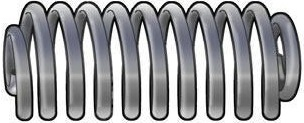
\includegraphics[width=0.4\textwidth]{spring3.jpg}\\
  \caption{ {\orange Hooke's law} models the properties of springs for small changes in length}
\end{figure}

\begin{columns}[onlytextwidth]
\begin{column}{0.5\textwidth}
  \centering
  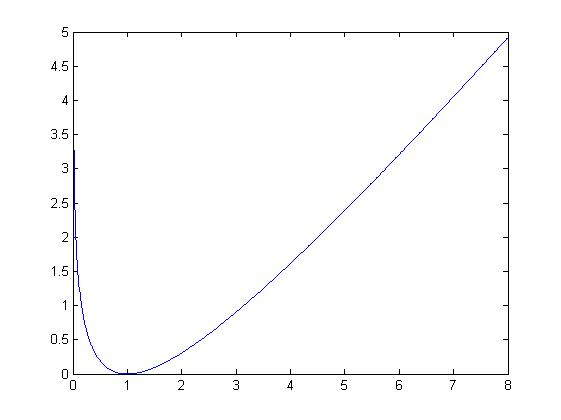
\includegraphics[width=\columnwidth]{error2.jpg}
\end{column}
\begin{column}{0.5\textwidth}
\begin{itemize}
  \item "Force" function:
$$F=\left\{  \begin{array}{ll}
                  x-1, & x\geq 1, \\
                  1-\frac{1}{x}, & x<1.
                \end{array}  \right. $$
then the energy function is h(x).
  \item Another proposal: \\$h(x)=x-(1+ln(x))$
\end{itemize}
\end{column}
\end{columns}
}

\frame{
\frametitle{Properties of new error function}
\begin{Theorem}
Suppose
$$
\begin{array}{ll}
f(x)&  = \sum\limits_{(i,j)\in S} h(\frac{\|x_i-x_j\|}{d_{ij}}) \\
 & =\sum\limits_{(i,j)\in S} \renewcommand{\arraystretch}{1.3}
 \left\{ \begin{array}{ll}
\frac{1}{2}(\frac{\|x_{i}-x_{j}\|}{d_{ij}}-1)^{2}, & \textrm{if } \|x_i-x_j\|\geq d_{ij}, \\
\frac{\|x_i-x_j\|}{d_{ij}} -1 -log(\frac{\|x_i-x_j\|}{d_{ij}}), & \textrm{otherwise}
\end{array} \right. \\
\end{array}
$$
let $N(i)=\{j:d_{ij}\neq 0\}$ denote the neighbours of point $i$, and $x=(x_1;x_2;\dots;x_n)$ is a column vector in $\mathbb{R}^{3n}$, then we have
$$\frac{\partial f}{\partial x_i}=\sum_{j\in N(i)} \renewcommand{\arraystretch}{1.3}
\left\{ \begin{array}{ll}
(\frac{1}{d_{ij}^2}-\frac{1}{d_{ij}\|x_i-x_j\|})(x_i-x_j), & \textrm{if } \|x_i-x_j\|\geq d_{ij}, \\
(\frac{1}{d_{ij}\|x_i-x_j\|}-\frac{1}{\|x_i-x_j\|^2})(x_i-x_j), & \textrm{otherwise}
\end{array} \right.,$$
\end{Theorem}
to be continued...
}

\frame{
\frametitle{Properties of new error function (cont'd)}
\begin{Theorem}
and for $p,q=1,2,3$,
$$\frac{\partial^2 f}{\partial x_{ip} \partial x_{jq}} =
\left\{ \begin{array}{rl}
\sum\limits_{j\in N(i)}\omega(x), & \textrm{if } i=j, \\
-\omega(x),& \textrm{if } i\neq j, \\
0,         & \textrm{otherwise}
\end{array} \right. $$
where
$$\omega(x) = \renewcommand{\arraystretch}{1.5}
    \left\{ \begin{array}{ll}
    \frac{1}{d_{ij}^2} - \frac{1}{d_{ij}\|x_i-x_j\|} + \frac{(x_{ip}-x_{jq})^2}{d_{ij}\|x_i-x_j\|^3}, & \textrm{if } \|x_i-x_j\|\geq d_{ij}, \\
    \frac{1}{d_{ij}\|x_i-x_j\|}- \frac{1}{\|x_i-x_j\|^2}- \frac{(x_{ip}-x_{jq})^2}{d_{ij}\|x_i-x_j\|^3} + \frac{(x_{ip}-x_{jq})^2}{\|x_i-x_j\|^4}, & \textrm{otherwise}. \\
    \end{array} \right.
$$
\end{Theorem}
}

\frame{
\frametitle{Our algorithm}
\begin{algorithm}[H]
\vspace{0.3cm}
Given: distance matrix D, i.e. $d_{ij}, (i,j)\in S$.
\begin{enumerate}[Step 1:]
  \item<2-> Find a clique of four points and determine their coordinates.
  \item<3-> {\red Choose} a point to be added, apply nonlinear least square to roughly locate the point.
  \item<4-> {\red Apply error minimization to these $l+1$ points}.
  \item<5-> Repeat {\blue Step 2-3} until all points are determined or no more points can be determined.
  \item<6-> {\red Apply error minimization to all the determined points}.
\end{enumerate}
\caption{Buildup-based Error Minimization Method for Distance Geometry Problem with sparse and noisy distances}
\end{algorithm}
}

\frame{
\frametitle{Algorithm details}
\begin{itemize}
  \item In {\blue Step 3}, we solve the following subproblem:
        \begin{equation*}
            \min_{x_j,x_k\in N(i)} f(x_j,x_k)
        \end{equation*}
        where $f$ is an error function.
  \item The subproblems are relatively very small, thus can be solved very quickly.\vskip6mm \pause
  \item In {\blue Step 5}, we solve
        \begin{equation*}
            \min_{x_1,x_2,\ldots,x_n} f(x_1,x_2,\ldots,x_n)
        \end{equation*}
  \item Since we can obtain very good starting point, we only exploit gradient method --- line search Barzilai-Borwein method to solve these problems.
\end{itemize}

}

\frame{
\frametitle{Buildup VS. our algorithm}
\begin{itemize}
  \item We re-use the same distance information (but only the given distances, not include calculated ones).
  \item In Buildup method equipped with nonlinear least square, if distances are noisy, then we have
    $$\|x_{i}-x_{j}\|=d_{ij}+e_{ij},$$ where $e_{ij}$ denotes noise.
    $$\Rightarrow 2\Tran{x_i}x_j = d_{in}^2 - d_{ij}^2 + d_{jn}^2 -  \boxed{{\blue(2d_{ij}e_{ij} + e_{ij}^2)}}$$
  \item So, our conclusion is:\\
       When the noises are large, {\blue $(d_{ij}e_{ij} + e_{ij}^2/2)$} should not be ignored, namely, solving $\Tran{X}X=D$ can not give a good solution to the original problem. But it can serve as a warm starting point to minimize an error function to obtain a better solution.
\end{itemize}
}

\section{Numerical experiments}
\frame{
\frametitle{Numerical experiments}
We simulate on real protein data, but the distance matrix is generated by us.
\begin{enumerate}
  \item Download PDB file from Internet to get the true positions of atoms.
  \item Use \emph{disk graph model} to generate distance matrix from these coordinates, with different cutoffs (6{\AA} or 5{\AA}) and variant noise level.
      $$d_{ij} = d_{ij} (1+noise*randn)$$
  \item Make numerical experiments with these distance matrices. Note that {\blue distances are the only information} we need to implement our algorithm.
  \item Examine the RMSD error of calculated positions with the true positions (in these experiments, we know these information).
  $$ RMSD(X,Y) = \min_{Q,T}\{ \|X-YQ-T\|_{F}/\sqrt{n}: \Tran{Q}Q=I\} $$
\end{enumerate}
}

\setlength{\tabcolsep}{3pt}
%\rowcolors{1}{white}{gray} % Colorful table
\frame{
\footnotesize{
\begin{table}
\begin{tabular}{crr|rrr|rrr|rrr|r}
  \hline
  ID   &  num & per  & \multicolumn{3}{c|}{degree} & \multicolumn{1}{c}{RMSD} & fval & & \multicolumn{3}{c|}{time(s)} & ndet \\
  \cline{4-6 } \cline{10-12}
       &      &      & max & min & ave &       &        & &   t1 & t2 & total &   \\
  \hline
  1PTQ &  402 & 5.46 &38 & 4 &21.9& 7.56e-02 &   2.40 &  3.20 &   0.6 &  0.1 &   0.8 &  402 \\
  1HOE &  558 & 4.05 &38 & 6 &22.6& 6.63e-02 &   3.53 &  4.68 &   0.8 &  0.2 &   0.9 &  558 \\
  1LFB &  641 & 3.40 &40 & 5 &21.8& 2.63e-01 &   4.00 &  5.01 &   1.0 &  0.3 &   1.3 &  641 \\
  1PHT &  811 & 3.35 &48 & 5 &27.1& 1.13e-01 &   6.16 &  7.81 &   1.8 &  0.4 &   2.1 &  806 \\
  1POA &  914 & 2.51 &39 & 4 &22.9& 1.11e-01 &   5.87 &  7.54 &   2.0 &  0.4 &   2.4 &  914 \\
  1AX8 & 1003 & 2.30 &39 & 5 &23.0& 2.06e-01 &   6.94 &  8.48 &   2.8 &  0.8 &   3.6 & 1003 \\
  1F39 & 1534 & 1.47 &40 & 5 &22.6& 1.08e-01 &   9.69 & 12.69 &   7.4 &  0.7 &   8.1 & 1534 \\
  1RGS & 2015 & 1.12 &41 & 3 &22.6& 1.64e-01 &  13.16 & 16.78 &  15.3 &  1.2 &  16.6 & 2010 \\
  1KDH & 2846 & 0.83 &43 & 4 &23.6& 3.19e-01 &  72.22 & 24.61 &  43.7 &  4.3 &  48.0 & 2846 \\
  1BPM & 3671 & 0.66 &42 & 3 &24.4& 1.17e-01 &  25.83 & 33.27 &  86.9 &  1.8 &  88.7 & 3668 \\
  1RHJ & 3740 & 0.65 &40 & 4 &24.4& 1.01e-01 &  26.39 & 34.15 &  90.4 &  2.5 &  92.9 & 3740 \\
  1HQQ & 3944 & 0.60 &40 & 3 &23.7& 1.75e-01 &  26.55 & 34.78 & 109.9 &  2.7 & 112.6 & 3938 \\
  1TOA & 4292 & 0.56 &39 & 3 &24.0& 8.73e-02 &  29.94 & 38.59 & 147.1 &  3.2 & 150.3 & 4280 \\
  1MQQ & 5681 & 0.44 &44 & 5 &25.2& 1.73e-01 &  42.44 & 53.18 & 323.1 &  5.5 & 328.6 & 5681 \\
  \hline
\end{tabular}
\caption{cutoff={\red 5}{\AA}, noise={\red 0.01}}
\end{table}
}
}

\frame{
\footnotesize{
\begin{table}
\begin{tabular}{crr|rrr|rr|rrr|r}
  \hline
  ID   &  num & per  & \multicolumn{3}{c|}{degree} & \multicolumn{1}{c}{RMSD} & fval & \multicolumn{3}{c|}{time(s)} & ndet \\
  \cline{4-6 } \cline{9-11}
       &      &      & max & min & ave &       &        &    t1 & t2 & total &   \\
  \hline
  1PTQ &  402 &  8.79& 61&  6& 35.3 & 4.96e-02 &  6.00 &  1.2 &  0.1&   1.3 &  402 \\
  1HOE &  558 &  6.55& 65& 11& 36.5 & 3.51e-02 &  8.90 &  1.8 &  0.2&   1.9 &  558 \\
  1LFB &  641 &  5.57& 59&  8& 35.7 & 5.53e-02 &  9.70 &  2.0 &  0.2&   2.2 &  641 \\
  1PHT &  811 &  5.37& 75&  7& 43.5 & 7.34e-02 & 15.82 &  4.1 &  0.3&   4.3 &  811 \\
  1POA &  914 &  4.07& 67&  8& 37.2 & 5.22e-02 & 15.04 &  3.9 &  0.3&   4.2 &  914 \\
  1AX8 & 1003 &  3.74& 59&  7& 37.5 & 4.25e-02 & 16.29 &  4.6 &  0.3&   5.0 & 1003 \\
  1F39 & 1534 &  2.43& 62&  7& 37.2 & 4.87e-02 & 25.55 & 10.6 &  0.5&  11.2 & 1534 \\
  1RGS & 2015 &  1.87& 66&  4& 37.7 & 6.28e-02 & 33.92 & 19.4 &  1.0&  20.4 & 2015 \\
  1KDH & 2846 &  1.36& 64&  5& 38.8 & 6.85e-02 & 49.81 & 47.7 &  1.6&  49.2 & 2846 \\
  1BPM & 3671 &  1.12& 64&  4& 40.9 & 4.24e-02 & 68.33 & 96.6 &  2.0&  98.6 & 3671 \\
  1RHJ & 3740 &  1.10& 61&  5& 41.2 & 3.21e-02 & 70.48 &103.1 &  2.1& 105.2 & 3740 \\
  1HQQ & 3944 &  1.00& 64&  5& 39.5 & 5.35e-02 & 69.81 &121.7 &  2.4& 124.1 & 3944 \\
  1TOA & 4292 &  0.94& 62&  4& 40.1 & 5.80e-02 & 77.70 &151.9 &  2.6& 154.6 & 4292 \\
  1MQQ & 5681 &  0.75& 66&  7& 42.4 & 3.34e-02 &110.56 &334.7 &  3.8& 338.5 & 5681 \\
  \hline
\end{tabular}
\caption{cutoff={\red 6}{\AA}, noise={\red 0.01}}
\end{table}
}
}

\frame{
\footnotesize{
\begin{table}
\begin{tabular}{crr|rrr|rr|rrr|r}
  \hline
  ID   &  num & per  & \multicolumn{3}{c|}{degree} & \multicolumn{1}{c}{RMSD} & fval & \multicolumn{3}{c|}{time(s)} & ndet \\
  \cline{4-6 } \cline{9-11}
       &      &      & max & min & ave &       &        &    t1 & t2 & total &   \\
  \hline
  1PTQ &  402 & 8.79&61&  6 &35.3& 2.44e-01&  149.64 &  2.4 &  0.3&   2.7& 402 \\
  1HOE &  558 & 6.55&65& 11 &36.5& 1.76e-01&  221.95 &  4.0 &  0.3&   4.3&  558 \\
  1LFB &  641 & 5.57&59&  8 &35.7& 2.46e-01&  241.74 &  4.6 &  0.5&   5.1&  641 \\
  1PHT &  811 & 5.37&75&  7 &43.5& 6.98e-01&  397.14 &  8.0 &  0.6&   8.6&  811 \\
  1POA &  914 & 4.07&67&  8 &37.2& 1.77e-01&  374.50 &  8.1 &  0.7&   8.8&  914 \\
  1AX8 & 1003 & 3.74&59&  7 &37.5& 1.89e-01&  405.16 &  9.3 &  0.7&  10.0& 1003 \\
  1F39 & 1534 & 2.43&62&  7 &37.2& 2.44e-01&  637.11 & 18.4 &  1.4&  19.8& 1534 \\
  1RGS & 2015 & 1.87&66&  4 &37.7& 3.13e-01&  845.78 & 30.4 &  3.5&  34.0& 2015 \\
  1KDH & 2846 & 1.36&64&  5 &38.8& 2.97e-01& 1240.51 & 69.7 &  4.1&  73.8& 2846 \\
  1BPM & 3671 & 1.12&64&  4 &40.9& 1.96e-01& 1706.83 &129.4 &  3.3& 132.7& 3671 \\
  1RHJ & 3740 & 1.10&61&  5 &41.2& 1.71e-01& 1760.82 &129.1 &  3.3& 132.4& 3740 \\
  1HQQ & 3944 & 1.00&64&  5 &39.5& 2.85e-01& 1744.20 &133.3 &  4.9& 138.2& 3944 \\
  1TOA & 4292 & 0.94&62&  4 &40.1& 2.36e-01& 1938.62 &182.6 &  5.0& 187.6& 4292 \\
  1MQQ & 5681 & 0.75&66&  7 &42.4& 2.04e-01& 2771.67 &400.3 &  6.1& 406.4& 5681 \\
  \hline
\end{tabular}
\caption{cutoff={\red 6}{\AA}, noise={\red 0.05}}
\end{table}
}
}

\frame{
\begin{figure}
  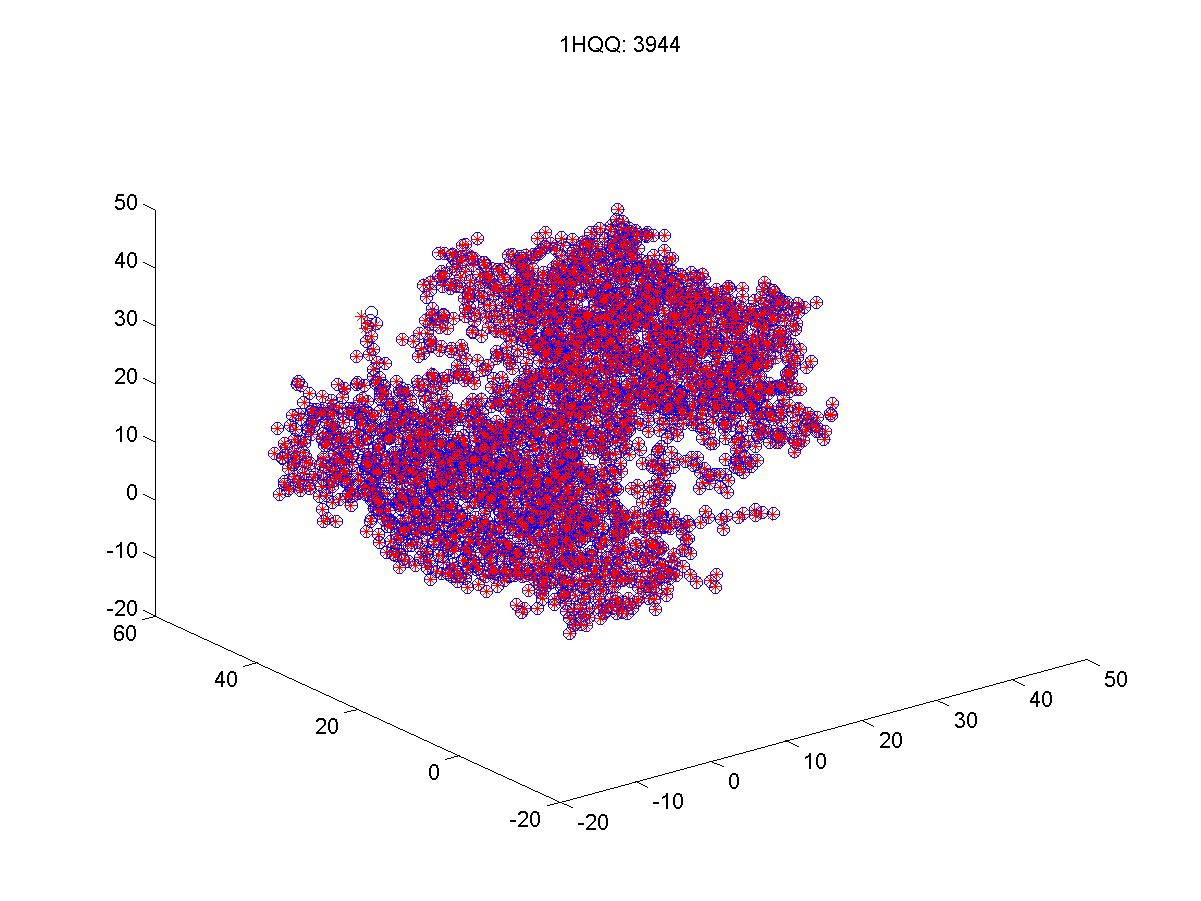
\includegraphics[width=\textwidth]{1HQQ61.jpg}
\end{figure}
}

\frame{
\begin{figure}
  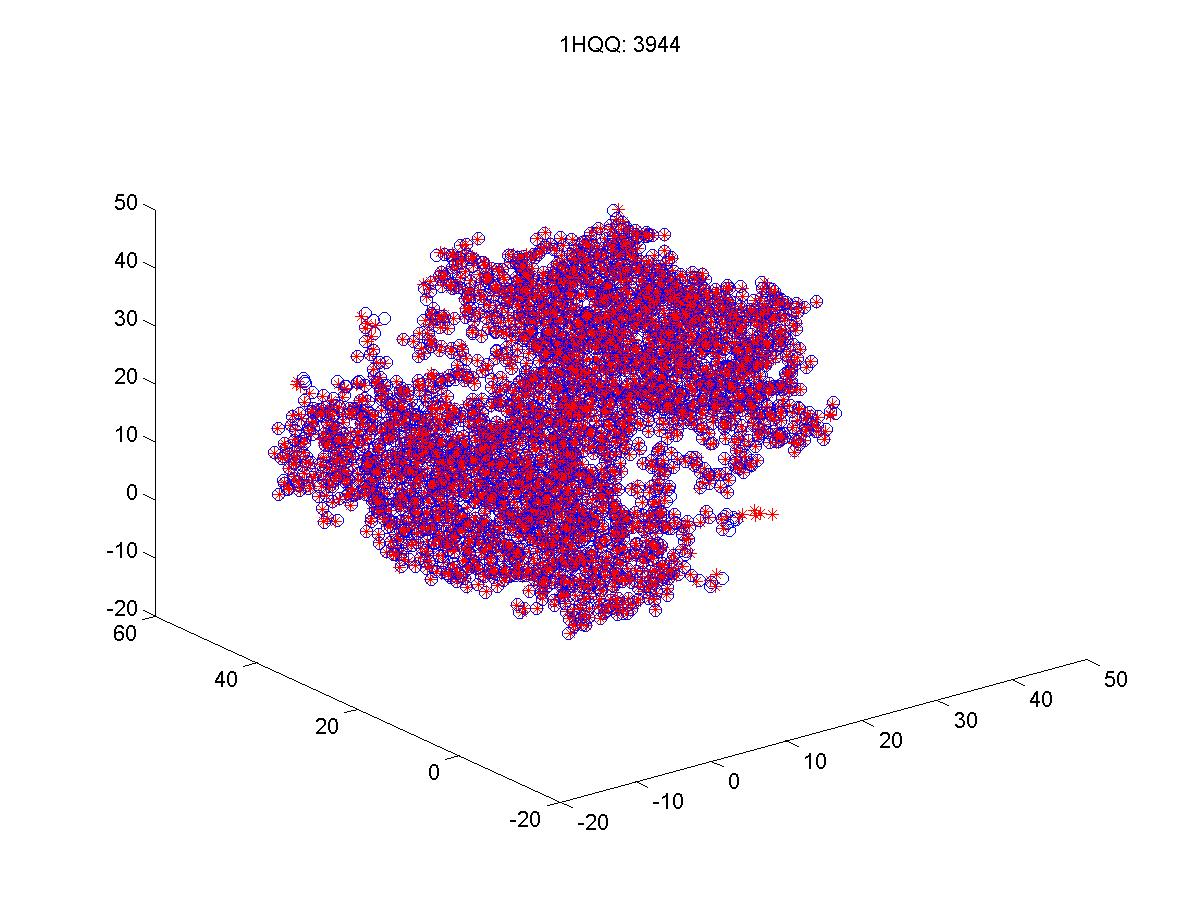
\includegraphics[width=\textwidth]{1HQQ65.jpg}
\end{figure}
}


\frame{
%\frametitle{Q \& A}
\begin{center}
  \Large{  \textsc{Thank you for your attention!}}  \\
  \vspace{0.2cm}
  {\blue szl@lsec.cc.ac.cn }
\end{center}
}

\end{CJK*}
\end{document}
